\chapter{La spectroscopie infrarouge}\label{ch:g11:infrared}

Sur une étagère de laboratoire se trouve un flacon de liquide incolore
dont l'étiquette a été arrachée. Ce pourrait être un \omterm{def:g11:functional-groups:alcohol}{alcool}, une \omterm{def:g11:functional-groups:carbonyl}{cétone}
ou un acide~: trois familles qui se ressemblent parfaitement dans un
flacon. Une goutte déposée sur le cristal d'un spectromètre infrarouge,
deux minutes d'attente, et un graphique apparaît à l'écran, qui répond à
la question. Les liaisons d'une \omterm{def:g7:atoms-and-molecules:molecule}{molécule} vibrent, et chaque sorte de
liaison absorbe la lumière infrarouge à des fréquences qui lui sont
propres~: un \omterm{def:g11:infrared:spectrum}{spectre infrarouge} est une liste des liaisons présentes.

\begin{recall}
Les \omterm{def:g11:functional-groups:functional-group}{groupes caractéristiques} et les familles
(\cref{ch:g11:functional-groups}). Un \omterm{def:g11:absorbance:spectrum}{spectre d'absorption} montre la
quantité de lumière qu'une substance absorbe à chaque longueur d'onde
(\cref{ch:g11:absorbance}). Les \omterm{def:g11:polarity-and-cohesion:hydrogen-bond}{liaisons hydrogène} relient les groupes
\ce{O-H} aux \omterm{def:g7:atoms-and-molecules:molecule}{molécules} voisines (\cref{ch:g11:polarity-and-cohesion}).
\end{recall}

\section{Les liaisons vibrent}

Une \omterm{def:g10:lewis-and-shape:covalent-bond}{liaison covalente} n'est pas rigide~: les deux \omterm{def:g7:atoms-and-molecules:atom}{atomes} vibrent, se
rapprochant et s'éloignant des millions de millions de fois par seconde,
comme deux boules reliées par un ressort. Un ressort plus raide (une
\omterm{def:g10:lewis-and-shape:multiple-bond}{liaison double} plutôt que simple) ou des boules plus légères (un \omterm{def:g7:atoms-and-molecules:atom}{atome}
d'hydrogène plutôt qu'un \omterm{def:g7:atoms-and-molecules:atom}{atome} de carbone) vibrent plus vite. Une
liaison peut absorber la lumière infrarouge dont la fréquence correspond
à sa propre vibration~: la lumière infrarouge, invisible à l'œil, a des
longueurs d'onde de quelques micromètres à quelques dizaines de
micromètres.

\begin{omfigure}
\begin{tikzpicture}[font=\small]
  \node[aC] (c) at (0,0) {};
  \node[aO] (o) at (2.2,0) {};
  \draw[decorate, decoration={coil, aspect=0.4, segment length=4pt,
    amplitude=4pt}, thick, black!60] (c.east) -- (o.west);
  \draw[<->, omProp, thick] (-0.9,0) -- (-0.45,0);
  \draw[<->, omProp, thick] (2.65,0) -- (3.1,0);
  \node[anchor=north] at (1.1,-0.5) {liaison étirée puis comprimée};
  \node[aO] (o1) at (5.3,0) {};
  \node[aH] (h1) at (6.7,0) {};
  \draw[decorate, decoration={coil, aspect=0.4, segment length=3pt,
    amplitude=3pt}, thick, black!60] (o1.east) -- (h1.west);
  \draw[<->, omProp, thick] (7.0,0) -- (7.7,0);
  \node[anchor=north, align=center] at (6.2,-0.5) {un atome d'hydrogène léger~:\\ vibration plus rapide};
\end{tikzpicture}

{\small Une liaison représentée comme un ressort entre deux boules. Sa
vibration a une fréquence fixée par la raideur de la liaison et les
masses des \omterm{def:g7:atoms-and-molecules:atom}{atomes}~; la lumière infrarouge de cette fréquence est
absorbée.}
\end{omfigure}

\begin{definition}[Nombre d'onde]\label{def:g11:infrared:wavenumber}
Le \emph{nombre d'onde}\index{nombre d'onde} $\sigma$ d'une lumière est
l'inverse de sa longueur d'onde, $\sigma = 1/\lambda$. En spectroscopie
infrarouge, on l'exprime en \si{cm^{-1}}~: c'est le nombre de longueurs
d'onde contenues dans un centimètre. Un nombre d'onde plus grand
correspond à une longueur d'onde plus courte et à une vibration plus
rapide.
\end{definition}

\begin{example}[D'un nombre d'onde à une longueur d'onde]\label{ex:g11:infrared:convert}
Une bande à $\sigma = \qty{2000}{cm^{-1}}$ correspond à
$\lambda = 1/2000 = \qty{5.0e-4}{cm} = \qty{5.0}{\micro m}$. Les \omterm{def:g11:infrared:spectrum}{spectres
infrarouges} s'étendent en général de \qty{4000}{cm^{-1}}
(\qty{2.5}{\micro m}) à \qty{500}{cm^{-1}} (\qty{20}{\micro m}).
\end{example}

\section{Lire un spectre infrarouge}

\begin{definition}[Spectre infrarouge, transmittance]\label{def:g11:infrared:spectrum}
La \emph{transmittance}\index{transmittance} $T$ d'un échantillon à un
\omterm{def:g11:infrared:wavenumber}{nombre d'onde} donné est le pourcentage de la lumière infrarouge qui le
traverse~: \qty{100}{\percent} si rien n'est absorbé. Le \emph{spectre
infrarouge}\index{spectre infrarouge} d'un composé est le graphique de
$T$ en fonction du \omterm{def:g11:infrared:wavenumber}{nombre d'onde}, tracé par convention avec des \omterm{def:g11:infrared:wavenumber}{nombres
d'onde} décroissants de gauche à droite.
\end{definition}

\begin{definition}[Bande d'absorption, empreinte digitale]\label{def:g11:infrared:band}
Une \emph{bande d'absorption}\index{bande d'absorption} est un creux de
la \omterm{def:g11:infrared:spectrum}{transmittance}~: la lumière de ces \omterm{def:g11:infrared:wavenumber}{nombres d'onde} est absorbée par une
liaison. Sa position indique de quelle liaison il s'agit~; sa largeur et
sa profondeur complètent le tableau. Au-dessous d'environ
\qty{1500}{cm^{-1}}, le spectre est encombré de bandes qui dépendent de
toute la \omterm{def:g7:atoms-and-molecules:molecule}{molécule}~: cette zone d'\emph{empreinte
digitale}\index{empreinte digitale} permet d'identifier un composé par
comparaison avec un spectre connu, mais se lit mal liaison par liaison.
\end{definition}

\begin{inthelab}[Enregistrer un spectre]
La plupart des spectromètres des lycées et des universités utilisent
aujourd'hui un petit cristal de diamant~: on dépose sur le cristal une
goutte de liquide, ou quelques grains de solide pressés par une pince,
et le faisceau infrarouge qui frôle sa surface sonde l'échantillon. On
enregistre d'abord le cristal propre (le «~fond~»), qui joue le rôle du
blanc. Entre deux échantillons, on nettoie le cristal avec un mouchoir
et un peu de \omterm{def:g6:solutions-and-solubility:solute}{solvant}.
\end{inthelab}

\section{Les bandes caractéristiques}

\begin{proposition}[Chaque type de liaison a sa bande]\label{prop:g11:infrared:bands}
% ledger: ir:OH-free, ir:OH-bonded, ir:OH-acid, ir:NH, ir:CH, ir:CO-aldehyde, ir:CO-ketone, ir:CO-ester, ir:CO-acid, ir:CC-double, ir:CO-single
Chaque type de liaison absorbe dans un domaine caractéristique de
\omterm{def:g11:infrared:wavenumber}{nombres d'onde}, presque le même d'une \omterm{def:g7:atoms-and-molecules:molecule}{molécule} à l'autre~:
\begin{center}
\small
\begin{tabular}{lll}
\hline
liaison & \omterm{def:g11:infrared:wavenumber}{nombre d'onde} (\si{cm^{-1}}) & aspect \\
\hline
\ce{O-H} libre (gaz, solution diluée) & vers 3600 & fine \\
\ce{O-H} lié (\omterm{def:g11:functional-groups:alcohol}{alcool} liquide) & 3300--3400 & large, intense \\
\ce{O-H} d'un \omterm{def:g11:functional-groups:carboxylic-acid}{acide carboxylique} & 2500--3300 & très large \\
\ce{N-H} d'une \omterm{def:g11:functional-groups:amine}{amine} & 3300--3500 & moyenne (deux bandes pour \ce{-NH2}) \\
\ce{C-H} d'une chaîne & 2850--2960 & intense \\
\ce{C=O} d'un \omterm{def:g11:functional-groups:carboxylic-acid}{ester} & vers 1735 & très intense, fine \\
\ce{C=O} d'un \omterm{def:g11:functional-groups:carbonyl}{aldéhyde} & vers 1730 & très intense, fine \\
\ce{C=O} d'une \omterm{def:g11:functional-groups:carbonyl}{cétone} & vers 1715 & très intense, fine \\
\ce{C=O} d'un \omterm{def:g11:functional-groups:carboxylic-acid}{acide carboxylique} & vers 1710 & très intense, plus large \\
\ce{C=C} & vers 1650 & moyenne \\
\ce{C-O} d'un \omterm{def:g11:functional-groups:alcohol}{alcool} & vers 1050 & intense \\
\hline
\end{tabular}
\end{center}
\end{proposition}

\begin{proof}
Ces domaines sont mesurés sur de nombreux composés. Ils se regroupent par
liaison parce que la vibration d'une liaison dépend surtout de la
liaison elle-même et de ses deux \omterm{def:g7:atoms-and-molecules:atom}{atomes}, peu du reste de la \omterm{def:g7:atoms-and-molecules:molecule}{molécule}.
\end{proof}

\begin{omfigure}
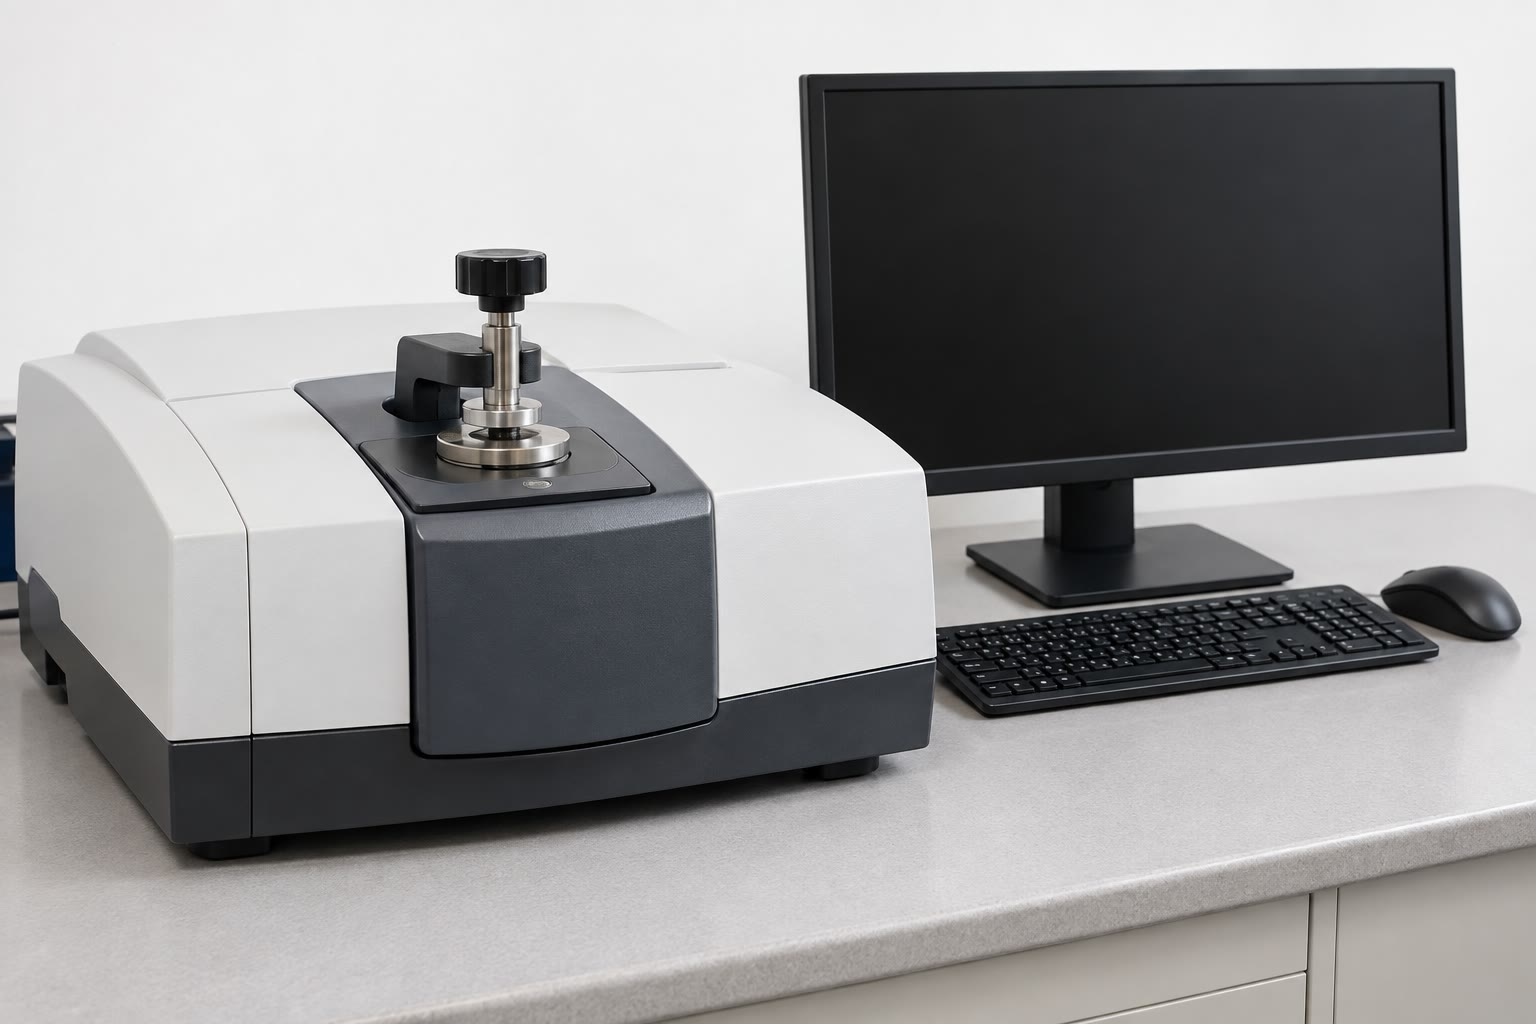
\includegraphics[width=0.48\linewidth]{images/book1/ai/g11-ftir.jpg}

{\small Un spectromètre infrarouge de paillasse, avec son cristal et sa
pince.}
\end{omfigure}

\begin{omfigure}
\begin{tikzpicture}[font=\small, x=0.0036cm, y=0.5cm]
  % wavenumber axis reversed: x = 4000 - sigma
  \fill[black!8] (2500,0.2) rectangle (3500,7.6);
  \node[font=\footnotesize, align=center, black!60] at (3000,6.8) {empreinte\\ digitale};
  \draw[->] (0,0) -- (3600,0) node[right] {$\sigma$};
  \foreach \s in {4000,3500,3000,2500,2000,1500,1000,500}
    \draw ({4000-\s},0) -- ({4000-\s},-0.15) node[below, font=\footnotesize] {\s};
  \node[below=12pt] at (1800,-0.3) {nombre d'onde (\si{cm^{-1}})};
  \foreach \a/\b/\y/\c/\l in {
      3600/3600/7/omDef/{\ce{O-H} libre},
      3300/3400/6/omDef/{\ce{O-H} lié},
      2500/3300/5/omThm/{\ce{O-H} acide},
      3300/3500/4/omMeth/{\ce{N-H}},
      2850/2960/3/black!60/{\ce{C-H}},
      1700/1740/2/omProp/{\ce{C=O}},
      1050/1050/1/black!45/{\ce{C-O}}} {
    \fill[\c, rounded corners=1pt] ({4000-\b-12},{\y-0.25}) rectangle ({4000-\a+12},{\y+0.25});
    \node[anchor=west, font=\footnotesize] at ({4000-\a+40},\y) {\l};
  }
\end{tikzpicture}

{\small Où absorbent les principales liaisons. Les bandes \ce{O-H} et
\ce{N-H} se trouvent à gauche, la bande \ce{C=O}, en général la plus
intense, vers \qty{1700}{cm^{-1}}~; au-dessous de \qty{1500}{cm^{-1}}
s'étend la zone d'\omterm{def:g11:infrared:band}{empreinte digitale}.}
\end{omfigure}

\begin{proposition}[Les liaisons hydrogène élargissent la bande O--H]\label{prop:g11:infrared:hbond}
% ledger: ir:OH-free, ir:OH-bonded, ir:ethanol-OH
Quand des groupes \ce{O-H} sont reliés par des \omterm{def:g11:polarity-and-cohesion:hydrogen-bond}{liaisons hydrogène}, comme
dans un \omterm{def:g11:functional-groups:alcohol}{alcool} liquide, leur bande est large et se situe à des \omterm{def:g11:infrared:wavenumber}{nombres
d'onde} plus faibles (vers 3300--\qty{3400}{cm^{-1}})~; sans \omterm{def:g11:polarity-and-cohesion:hydrogen-bond}{liaisons
hydrogène}, comme dans le gaz, elle est fine et vers
\qty{3600}{cm^{-1}}.
\end{proposition}

\begin{proof}
Admis~: une \omterm{def:g11:polarity-and-cohesion:hydrogen-bond}{liaison hydrogène} tire sur l'\omterm{def:g7:atoms-and-molecules:atom}{atome} d'hydrogène et affaiblit
la liaison \ce{O-H}, qui vibre plus lentement~; et comme chaque \omterm{def:g7:atoms-and-molecules:molecule}{molécule}
est liée un peu différemment, la bande s'étale sur un domaine.
\end{proof}

\section{Identifier des groupes caractéristiques}


\begin{method}[Lire un spectre infrarouge]\label{met:g11:infrared:reading}
\begin{enumerate}
  \item Regarder d'abord au-dessus de \qty{1500}{cm^{-1}}~; garder la zone
        d'\omterm{def:g11:infrared:band}{empreinte digitale} pour une comparaison avec des spectres
        connus.
  \item Vers \qty{1700}{cm^{-1}}~: une bande très intense signale un
        groupe \ce{C=O} (\omterm{def:g11:functional-groups:carbonyl}{aldéhyde}, \omterm{def:g11:functional-groups:carbonyl}{cétone}, acide, \omterm{def:g11:functional-groups:carboxylic-acid}{ester}, \omterm{def:g11:functional-groups:amine}{amide}).
  \item Entre 2500 et \qty{3700}{cm^{-1}}~: une bande large vers
        \qty{3350}{cm^{-1}} signale un \ce{O-H} d'\omterm{def:g11:functional-groups:alcohol}{alcool}~; une bande très
        large de 2500 à \qty{3300}{cm^{-1}} accompagnée d'un \ce{C=O}
        signale un \omterm{def:g11:functional-groups:carboxylic-acid}{acide carboxylique}~; des bandes moyennes à
        3300--\qty{3500}{cm^{-1}} signalent des \ce{N-H}.
  \item Combiner avec la \omterm{def:g11:organic-skeletons:formulas}{formule brute} pour choisir la famille, puis
        vérifier avec la position de la bande \ce{C=O} s'il y en a une.
\end{enumerate}
\end{method}

\begin{omfigure}
\newcommand{\irpanel}[2]{%
\begin{tikzpicture}
\begin{axis}[width=0.96\linewidth, height=3.9cm, x dir=reverse, xmin=500,
    xmax=4000, ymin=0, ymax=105, xtick={4000,3000,2000,1000},
    /pgf/number format/1000 sep={},
    ytick={0,50,100}, tick label style={font=\scriptsize},
    label style={font=\scriptsize}, ylabel={$T$ (\%)}, axis lines*=left,
    title={\small #2}, title style={yshift=-4pt}]
  \addplot[thick, omDef] table[x=sigma, y=#1] {figdata/out/grade-11-infrared.dat};
\end{axis}
\end{tikzpicture}}
\begin{minipage}{0.49\linewidth}\irpanel{ethanolL}{A~: éthanol (liquide)}\end{minipage}\hfill
\begin{minipage}{0.49\linewidth}\irpanel{ethanolG}{B~: éthanol (gaz)}\end{minipage}

\begin{minipage}{0.49\linewidth}\irpanel{propanone}{C~: propanone}\end{minipage}\hfill
\begin{minipage}{0.49\linewidth}\irpanel{acid}{D~: acide éthanoïque}\end{minipage}

\begin{minipage}{0.49\linewidth}\irpanel{ester}{E~: éthanoate d'éthyle}\end{minipage}\hfill
\begin{minipage}{0.49\linewidth}\irpanel{amine}{F~: éthanamine}\end{minipage}

{\small \omterm{def:g11:infrared:spectrum}{Spectres infrarouges} de six composés, \omterm{def:g11:infrared:wavenumber}{nombre d'onde} en
\si{cm^{-1}} (décroissant vers la droite). Seules les bandes étudiées
dans le chapitre sont tracées~; leurs positions proviennent de spectres
mesurés et de tables, leurs formes d'un modèle simple.}
\end{omfigure}

\begin{example}[Lire les six spectres]\label{ex:g11:infrared:six}
% ledger: ir:OH-bonded, ir:ethanol-OH, ir:CO-ketone, ir:OH-acid, ir:CO-acid, ir:CO-ester, ir:ethylethanoate-COC, ir:NH
L'éthanol (A) présente une large bande \ce{O-H} vers \qty{3350}{cm^{-1}},
les bandes \ce{C-H} juste au-dessous de \qty{3000}{cm^{-1}} et une
bande \ce{C-O} intense vers \qty{1050}{cm^{-1}}, mais rien vers
\qty{1700}{cm^{-1}}. Dans le gaz (B), sa bande \ce{O-H} devient une raie
fine à \qty{3666}{cm^{-1}}. La propanone (C) n'a pas de bande \ce{O-H}
mais un \ce{C=O} très intense à \qty{1715}{cm^{-1}}. L'acide éthanoïque
(D) présente les deux~: une énorme bande \ce{O-H} de 2500 à
\qty{3300}{cm^{-1}} et un \ce{C=O} à \qty{1710}{cm^{-1}}. L'éthanoate
d'éthyle (E) a son \ce{C=O} à \qty{1735}{cm^{-1}} et un \ce{C-O} intense
vers \qty{1240}{cm^{-1}}, et pas de \ce{O-H}. L'éthanamine (F) présente
deux bandes \ce{N-H} moyennes au-dessus de \qty{3300}{cm^{-1}}.
\end{example}

\section{Exercices}

\begin{exercise}[$\star$]\label{exo:g11:infrared:1}
Convertir en longueur d'onde, en micromètres~: $\sigma = \qty{3300}{cm^{-1}}$
et $\sigma = \qty{1050}{cm^{-1}}$. Laquelle correspond à la vibration la
plus rapide~?
\end{exercise}

\begin{exercise}[$\star$]\label{exo:g11:infrared:2}
Une longueur d'onde de \qty{10}{\micro m} est absorbée. Donner le \omterm{def:g11:infrared:wavenumber}{nombre
d'onde} en \si{cm^{-1}}.
\end{exercise}

\begin{exercise}[$\star$]\label{exo:g11:infrared:3}
Quelle liaison absorbe~: vers \qty{1715}{cm^{-1}}~; vers
\qty{3350}{cm^{-1}} (bande large)~; entre 2850 et \qty{2960}{cm^{-1}}~?
\end{exercise}

\begin{exercise}[$\star$]\label{exo:g11:infrared:4}
Sur le spectre C (propanone), repérer la bande la plus intense. À quelle
liaison appartient-elle~?
\end{exercise}

\begin{exercise}[$\star$]\label{exo:g11:infrared:5}
Pourquoi trace-t-on un \omterm{def:g11:infrared:spectrum}{spectre infrarouge} avec un axe de \omterm{def:g11:infrared:spectrum}{transmittance},
les bandes pointant vers le bas~? Que signifie $T = \qty{100}{\percent}$~?
\end{exercise}

\begin{exercise}[$\star\star$]\label{exo:g11:infrared:6}
Un composé \ce{C4H8O} présente une bande très intense à
\qty{1715}{cm^{-1}} et aucune bande au-dessus de \qty{3000}{cm^{-1}}. Un
autre, \ce{C4H10O}, présente une bande large vers \qty{3350}{cm^{-1}} et
aucune vers \qty{1700}{cm^{-1}}. À quelles familles appartiennent-ils~?
Proposer un nom pour chacun.
\end{exercise}

\begin{exercise}[$\star\star$]\label{exo:g11:infrared:7}
Expliquer pourquoi la bande \ce{O-H} de l'acide éthanoïque est si large,
plus large encore que celle de l'éthanol liquide.
\end{exercise}

\begin{exercise}[$\star\star$]\label{exo:g11:infrared:8}
Comparer les spectres A et B de l'éthanol. Qu'est-ce qui change, et
pourquoi~?
\end{exercise}

\begin{exercise}[$\star\star$]\label{exo:g11:infrared:9}
Le propanal et la propanone ont tous deux pour formule \ce{C3H6O}. Tous
deux présentent une bande \ce{C=O} intense. L'infrarouge peut-il les
distinguer à partir de cette seule bande~? Qu'est-ce qui pourrait
aider~?
\end{exercise}

\begin{exercise}[$\star\star$]\label{exo:g11:infrared:10}
Un composé présente une bande intense à \qty{1735}{cm^{-1}}, une bande
intense vers \qty{1240}{cm^{-1}} et rien au-dessus de
\qty{3000}{cm^{-1}}. Sa formule est \ce{C4H8O2}. Quelle famille~?
L'acide éthanoïque est-il possible~? Et l'acide butanoïque~?
\end{exercise}

\begin{exercise}[$\star\star$]\label{exo:g11:infrared:11}
À lequel des six spectres ressemblerait le plus celui d'une \omterm{def:g7:atoms-and-molecules:molecule}{molécule} de
propan-1-ol~? Et celui de l'acide propanoïque~? Expliquer.
\end{exercise}

\begin{exercise}[$\star\star\star$]\label{exo:g11:infrared:12}
Le propan-2-ol peut être oxydé en propanone. Une élève suit la réaction
en enregistrant les spectres d'échantillons prélevés toutes les dix
minutes. Décrire l'évolution des spectres. Comment sait-elle que la
réaction est terminée~?
\end{exercise}

\begin{exercise}[$\star\star\star$]\label{exo:g11:infrared:13}
L'acide butanoïque et l'éthanoate d'éthyle sont \omterm{def:g11:organic-skeletons:isomer}{isomères}, \ce{C4H8O2}.
Décrire deux différences entre leurs \omterm{def:g11:infrared:spectrum}{spectres infrarouges}, et les
expliquer.
\end{exercise}

\begin{exercise}[$\star\star\star$]\label{exo:g11:infrared:14}
Un échantillon d'éthanoate d'éthyle présente, en plus des bandes
attendues, une faible bande large vers \qty{3350}{cm^{-1}}. Proposer deux
impuretés qui pourraient en être la cause (penser à la façon dont on
fabrique les \omterm{def:g11:functional-groups:carboxylic-acid}{esters}, et à l'\omterm{def:g4:air-a-mixture-of-gases:air}{air}). Comment pourrait-on contrôler
l'échantillon~?
\end{exercise}

\begin{exercise}[$\star\star\star$]\label{exo:g11:infrared:15}
La bande \ce{C=O} des \omterm{def:g11:functional-groups:carbonyl}{cétones} se situe vers \qty{1715}{cm^{-1}}, celle
d'un \ce{C=C} vers \qty{1650}{cm^{-1}}, et la bande \ce{C-O} vers
\qty{1050}{cm^{-1}}. À l'aide de l'image des deux boules reliées par un
ressort, expliquer pourquoi une \omterm{def:g10:lewis-and-shape:multiple-bond}{liaison double} \ce{C=O} vibre plus vite
qu'une liaison simple \ce{C-O}. Pourquoi les bandes \ce{O-H}, \ce{N-H}
et \ce{C-H} sont-elles toutes à des \omterm{def:g11:infrared:wavenumber}{nombres d'onde} élevés~?
\end{exercise}

\section{Problème~: trois flacons sans étiquette}

\begin{problem}[{Problème du week-end --- trois flacons ont perdu leurs
étiquettes~: lequel est lequel, et quelle longueur d'onde la cétone
absorbe-t-elle le plus~?}]
\label{pb:g11:infrared:1}
% ledger: ir:OH-bonded, ir:OH-acid, ir:CO-ketone, ir:CO-acid, ir:CO-single
Trois flacons de liquide incolore ont perdu leurs étiquettes. Selon
l'inventaire, ils contiennent de l'éthanol, de la propanone et de
l'acide éthanoïque. On enregistre leurs spectres~: le flacon 1 donne un
spectre semblable à A, le flacon 2 à D, le flacon 3 à C.

\medskip
\noindent\textbf{Partie I --- Les candidats.}
\begin{enumerate}
  \item Écrire les \omterm{def:g11:organic-skeletons:formulas}{formules semi-développées} de l'éthanol, de la
        propanone et de l'acide éthanoïque.
  \item Donner leurs \omterm{def:g11:organic-skeletons:formulas}{formules brutes}.
  \item Nommer le \omterm{def:g11:functional-groups:functional-group}{groupe caractéristique} de chacun.
  \item Quelles liaisons de chacun devraient donner une bande au-dessus
        de \qty{1500}{cm^{-1}}~?
\end{enumerate}

\medskip
\noindent\textbf{Partie II --- Les spectres.}
\begin{enumerate}[resume]
  \item Flacon 1~: y a-t-il une bande \ce{C=O}~? Une bande \ce{O-H}~?
        Quel composé est-ce~?
  \item Flacon 2~: décrire ses deux caractéristiques les plus marquées.
        Quel composé~?
  \item Flacon 3~: quel composé~? Quelle bande permet de trancher~?
  \item L'odeur aurait-elle permis de les distinguer~? Pourquoi vaut-il
        mieux ne pas essayer~?
  \item Pourquoi la bande \ce{O-H} du flacon 2 est-elle plus large que
        celle du flacon 1~?
\end{enumerate}

\medskip
\noindent\textbf{Partie III --- Les \omterm{def:g11:organic-skeletons:isomer}{isomères}.}
\begin{enumerate}[resume]
  \item Le méthoxyméthane est un \omterm{def:g11:organic-skeletons:isomer}{isomère} de l'éthanol. Écrire sa formule.
        Quelle bande de l'éthanol manquerait à son spectre~?
  \item Le propanal est un \omterm{def:g11:organic-skeletons:isomer}{isomère} de la propanone. Quelle bande ont-ils
        en commun~? Où se situe-t-elle pour chacun~?
  \item Le méthanoate de méthyle, \ce{HCOO-CH3}, est un \omterm{def:g11:organic-skeletons:isomer}{isomère} de l'acide
        éthanoïque. Quelle bande de l'acide manquerait~? Où se situerait
        sa bande \ce{C=O}~?
  \item Pourquoi une \omterm{def:g11:organic-skeletons:formulas}{formule brute} seule ne permet-elle pas d'identifier
        un composé, alors que la formule et le spectre réunis le
        permettent en général~?
\end{enumerate}

\medskip
\noindent\textbf{Partie IV --- La longueur d'onde.}
\begin{enumerate}[resume]
  \item Quel est le \omterm{def:g11:infrared:wavenumber}{nombre d'onde} de la bande la plus intense de la
        propanone~?
  \item L'exprimer en \si{m^{-1}}.
  \item Calculer la longueur d'onde absorbée, en mètres, puis en
        micromètres.
  \item Cette lumière est-elle visible~? À quel type de rayonnement
        appartient-elle~?
  \item Faire de même pour la bande \ce{C-O} de l'éthanol vers
        \qty{1050}{cm^{-1}}.
  \item Laquelle des deux liaisons vibre le plus vite~?
  \item Donner la réponse finale~: quelle longueur d'onde la liaison
        \ce{C=O} de la propanone absorbe-t-elle le plus fortement~?
\end{enumerate}
\end{problem}
